
\section{Body}

\subsection{Part 1: Pendulum}

\begin{frame}
\frametitle{Part 1: Pendulum}
\center
The Formula for the time period of a pendulum is: \cite{pendulum_time_period}\pause
\begin{equation}
	T = 2\pi \sqrt {\frac{l}{g}}
\end{equation}
\begin{flushleft}
\begin{itemize}
\pause
\item Here $ l $ is the length of thread from bob to pivot point and $ g $ is the acceleration due to gravity($ \approx 9.81 m/sec^2 $)\pause
\item $ g $ is the acceleration due to gravity.\\ \pause
\item $ v_x $ id the initial velocity of ball in x-direction (No acceleration in x-direction).\pause
\end{itemize}
\end{flushleft}
\begin{figure}
		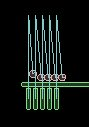
\includegraphics[width=2.5cm,height=2.5cm,keepaspectratio]{pendulum.jpg}
\end{figure}
\end{frame}

\subsection{Part 2: Flying Ball}

\begin{frame}
\frametitle{Part 2: Flying Ball}
\center
The equation of motion of a ball in free fall is: \cite{freeFall}\\
\begin{equation}
	s_y = u_y t + \frac{1}{2}gt^2
\end{equation}
\begin{equation}
	s_x = v_x t
\end{equation}
\begin{flushleft}
\begin{itemize}
\item $ s_y $ is the displacement in the y direction and $ s_x $ is the dispacement in x direction.\pause \\
\item $ g $ is the acceleration due to gravity.\pause \\
\item $ v_x $ id the initial velocity of ball in x-direction (No acceleration in x-direction).\pause
\end{itemize}
\end{flushleft}
\begin{figure}
		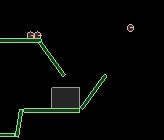
\includegraphics[width=2.5cm,height=2.5cm,keepaspectratio]{flyingball.jpg}
\end{figure}
\end{frame}


\subsection{Part 3: Collision}
\begin{frame}
	\frametitle{Part 3: Collision}
	\center
	Collision is dependent on the surfaces involved to a large extent. The principle equations involved are:\cite{Collision} \pause \\
	
	\begin{equation}
		m_1 v_{i1} + m_2 v_{i2} = m_1 v_{f1} + m_2 v_{f2}
	\end{equation}
	\pause
	\begin{equation}
		e = \frac{v_{f2} - v_{f1}}{v_{i2}-v_{i1}}
	\end{equation}	
	\pause
	\begin{columns}
	\column{0.7\textwidth}	
		\begin{itemize}
			\item e is a constant for two surfaces and is called  coefficient of restituion .It is dimensionless.\\\pause
			%\item $ m_1 $ and $ m_2 $ are the masses of bodies 1 and 2.\\
			\item $ v_{1i} $ ,$ v_{1f} $ , $ v_{2i} $ and $ v_{2f} $ are the velocities of body 1 and body 2 before and after the collision.\\\pause
		\end{itemize}
	\column{0.3\textwidth}
		\begin{figure}
			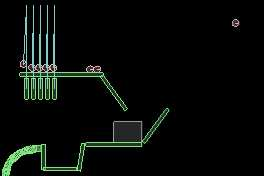
\includegraphics[width=2.5cm,height=2.5cm]{collision.jpg}
		\end{figure}
	\end{columns}
\end{frame}
